%File: anonymous-submission-latex-2024.tex
\documentclass[letterpaper]{article} % DO NOT CHANGE THIS
\usepackage[submission]{aaai24}  % DO NOT CHANGE THIS
\usepackage{times}  % DO NOT CHANGE THIS
\usepackage{helvet}  % DO NOT CHANGE THIS
\usepackage{courier}  % DO NOT CHANGE THIS
\usepackage[hyphens]{url}  % DO NOT CHANGE THIS
\usepackage{graphicx} % DO NOT CHANGE THIS
\urlstyle{rm} % DO NOT CHANGE THIS
\def\UrlFont{\rm}  % DO NOT CHANGE THIS
\usepackage{natbib}  % DO NOT CHANGE THIS AND DO NOT ADD ANY OPTIONS TO IT
\usepackage{caption} % DO NOT CHANGE THIS AND DO NOT ADD ANY OPTIONS TO IT
\frenchspacing  % DO NOT CHANGE THIS
\setlength{\pdfpagewidth}{8.5in} % DO NOT CHANGE THIS
\setlength{\pdfpageheight}{11in} % DO NOT CHANGE THIS
%
% These are recommended to typeset algorithms but not required. See the subsubsection on algorithms. Remove them if you don't have algorithms in your paper.
\usepackage{algorithm}
% \usepackage{algorithmic}

%
% These are are recommended to typeset listings but not required. See the subsubsection on listing. Remove this block if you don't have listings in your paper.
% \usepackage{newfloat}
% \usepackage{listings}
% \DeclareCaptionStyle{ruled}{labelfont=normalfont,labelsep=colon,strut=off} % DO NOT CHANGE THIS
% \lstset{%
% 	basicstyle={\footnotesize\ttfamily},% footnotesize acceptable for monospace
% 	numbers=left,numberstyle=\footnotesize,xleftmargin=2em,% show line numbers, remove this entire line if you don't want the numbers.
% 	aboveskip=0pt,belowskip=0pt,%
% 	showstringspaces=false,tabsize=2,breaklines=true}
% \floatstyle{ruled}
% \newfloat{listing}{tb}{lst}{}
% \floatname{listing}{Listing}
%
% Keep the \pdfinfo as shown here. There's no need
% for you to add the /Title and /Author tags.
\pdfinfo{
/TemplateVersion (2024.1)
}

\usepackage{amsfonts}       % blackboard math symbols
\usepackage{amsmath}
\usepackage{amsthm}
\usepackage{caption}
\usepackage{graphicx}
\usepackage{algpseudocode}
\usepackage{import}
\usepackage{booktabs}
\usepackage{longtable}
\usepackage{array}
\usepackage{multirow}
\usepackage{placeins}


% Numbered Environments:
\newtheorem{definition}{Definition}[section]
\newtheorem{question}{Research Question}[section]

% Bibliography
% \bibliographystyle{unsrtnat}
% \setcitestyle{numbers,square,comma}

% Algorithm
\renewcommand{\algorithmicrequire}{\textbf{Input:}}
\renewcommand{\algorithmicensure}{\textbf{Output:}}

% DISALLOWED PACKAGES
% \usepackage{authblk} -- This package is specifically forbidden
% \usepackage{balance} -- This package is specifically forbidden
% \usepackage{color (if used in text)
% \usepackage{CJK} -- This package is specifically forbidden
% \usepackage{float} -- This package is specifically forbidden
% \usepackage{flushend} -- This package is specifically forbidden
% \usepackage{fontenc} -- This package is specifically forbidden
% \usepackage{fullpage} -- This package is specifically forbidden
% \usepackage{geometry} -- This package is specifically forbidden
% \usepackage{grffile} -- This package is specifically forbidden
% \usepackage{hyperref} -- This package is specifically forbidden
% \usepackage{navigator} -- This package is specifically forbidden
% (or any other package that embeds links such as navigator or hyperref)
% \indentfirst} -- This package is specifically forbidden
% \layout} -- This package is specifically forbidden
% \multicol} -- This package is specifically forbidden
% \nameref} -- This package is specifically forbidden
% \usepackage{savetrees} -- This package is specifically forbidden
% \usepackage{setspace} -- This package is specifically forbidden
% \usepackage{stfloats} -- This package is specifically forbidden
% \usepackage{tabu} -- This package is specifically forbidden
% \usepackage{titlesec} -- This package is specifically forbidden
% \usepackage{tocbibind} -- This package is specifically forbidden
% \usepackage{ulem} -- This package is specifically forbidden
% \usepackage{wrapfig} -- This package is specifically forbidden
% DISALLOWED COMMANDS
% \nocopyright -- Your paper will not be published if you use this command
% \addtolength -- This command may not be used
% \balance -- This command may not be used
% \baselinestretch -- Your paper will not be published if you use this command
% \clearpage -- No page breaks of any kind may be used for the final version of your paper
% \columnsep -- This command may not be used
% \newpage -- No page breaks of any kind may be used for the final version of your paper
% \pagebreak -- No page breaks of any kind may be used for the final version of your paperr
% \pagestyle -- This command may not be used
% \tiny -- This is not an acceptable font size.
% \vspace{- -- No negative value may be used in proximity of a caption, figure, table, section, subsection, subsubsection, or reference
% \vskip{- -- No negative value may be used to alter spacing above or below a caption, figure, table, section, subsection, subsubsection, or reference

\setcounter{secnumdepth}{2} %May be changed to 1 or 2 if section numbers are desired.

% The file aaai24.sty is the style file for AAAI Press
% proceedings, working notes, and technical reports.
%

% Title

% Your title must be in mixed case, not sentence case.
% That means all verbs (including short verbs like be, is, using,and go),
% nouns, adverbs, adjectives should be capitalized, including both words in hyphenated terms, while
% articles, conjunctions, and prepositions are lower case unless they
% directly follow a colon or long dash
\title{Faithful Model Explanations through\\
Energy-Constrained Conformal Counterfactuals}
\author{
    %Authors
    % All authors must be in the same font size and format.
    Written by AAAI Press Staff\textsuperscript{\rm 1}\thanks{With help from the AAAI Publications Committee.}\\
    AAAI Style Contributions by Pater Patel Schneider,
    Sunil Issar,\\
    J. Scott Penberthy,
    George Ferguson,
    Hans Guesgen,
    Francisco Cruz\equalcontrib,
    Marc Pujol-Gonzalez\equalcontrib
}
\affiliations{
    %Afiliations
    \textsuperscript{\rm 1}Association for the Advancement of Artificial Intelligence\\
    % If you have multiple authors and multiple affiliations
    % use superscripts in text and roman font to identify them.
    % For example,

    % Sunil Issar\textsuperscript{\rm 2},
    % J. Scott Penberthy\textsuperscript{\rm 3},
    % George Ferguson\textsuperscript{\rm 4},
    % Hans Guesgen\textsuperscript{\rm 5}
    % Note that the comma should be placed after the superscript

    1900 Embarcadero Road, Suite 101\\
    Palo Alto, California 94303-3310 USA\\
    % email address must be in roman text type, not monospace or sans serif
    proceedings-questions@aaai.org
%
% See more examples next
}

%Example, Single Author, ->> remove \iffalse,\fi and place them surrounding AAAI title to use it
% \iffalse
% \title{My Publication Title --- Single Author}
% \author {
%     Author Name
% }
% \affiliations{
%     Affiliation\\
%     Affiliation Line 2\\
%     name@example.com
% }
% \fi

% \iffalse
% %Example, Multiple Authors, ->> remove \iffalse,\fi and place them surrounding AAAI title to use it
% \title{My Publication Title --- Multiple Authors}
% \author {
%     % Authors
%     First Author Name\textsuperscript{\rm 1},
%     Second Author Name\textsuperscript{\rm 2},
%     Third Author Name\textsuperscript{\rm 1}
% }
% \affiliations {
%     % Affiliations
%     \textsuperscript{\rm 1}Affiliation 1\\
%     \textsuperscript{\rm 2}Affiliation 2\\
%     firstAuthor@affiliation1.com, secondAuthor@affilation2.com, thirdAuthor@affiliation1.com
% }
% \fi

\begin{document}

We thank the reviewers for their thoughtful comments and are glad with the overall positive response. 

\subsection*{Reviewer \#1}

\subsubsection{1. Experiment results: linguistic explanation.}  

We will add a linguistic explanation in Section 6 where we highlight that \textit{ECCCo} produces plausible counterfactuals iff the classifier itself has learned plausible explanations for the data. It thus avoids the risk of generating plausible but potentially misleading explanations for models that are highly susceptible to implausible explanations.

\subsubsection{2. Core innovation: more visualizations.} 

Figure~\ref{fig:poc} shows the relationship between implausibility and the energy constraint for MNIST data. As expected, this relationship is positive and the size of the relationship depends positively on the model's generative property (the observed relationships are stronger for joint energy models). We will add such images for all datasets to the appendix.  We note that our final benchmark results involve around 1.5 million counterfactuals per dataset (not including grid searches).

\begin{figure}[h]
    \centering
    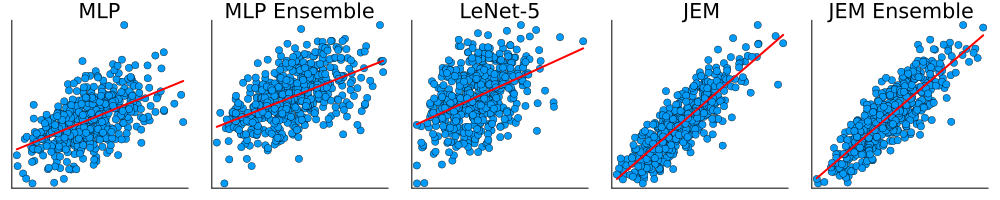
\includegraphics[width=\linewidth]{../../www/dist_energy.png}
    \caption{The L2 distance of randomly drawn MNIST images with Gaussian perturbations from unperturbed images in the target class (horizontal axis) plotted against their energy-constrained score, i.e. target logit (vertical axis).}\label{fig:poc}
\end{figure}  

\subsubsection{3. Structural clarity.} 

To facilitate comprehension, we will follow the reviewer's advice and add a systematic flowchart either in the appendix or in place of Figure 2.

\subsection*{Reviewer \#2}

\subsubsection{4. Why use an embedding?}

There are two main reasons for using a low-dimensional latent embedding: firstly, to help with plausibility and, secondly, to reduce computational costs. The latter is not currently made explicit in the paper and we will add this in Section 5. The former is discussed in the context of the results for \textit{ECCCo+} in Section 6.3, but we will highlight the following rationale:

There is indeed a tradeoff between plausibility and faithfulness through the introduction of bias: plausibility is improved because counterfactuals are insensitive to variation captured by higher-order principal components. Intuitively, the generated counterfactuals are therefore less noisy. We think that the bias introduced by PCA may be acceptable, precisely because it `will not add any information on the input distribution' as the reviewer correctly points out. To maintain faithfulness, we want to avoid adding any information through surrogate models as much as possible.

\subsubsection{5. What is `epsilon' and `s'?}

From the paper: `[...] the step-size $\epsilon_j$ is typically polynomially decayed.' Intuitively, $\epsilon_j$ determines the size of gradient updates and random noise in each iteration of SGLD.

Regarding $s(\cdot)$, this was an oversight. In the appendix we explain that `[the calibration dataset] is then used to compute so-called nonconformity scores: $\mathcal{S}=\{s(\mathbf{x}_i,\mathbf{y}_i)\}_{i \in \mathcal{D}_{\text{cal}}}$ where $s: (\mathcal{X},\mathcal{Y}) \mapsto \mathbb{R}$ is referred to as \textit{score function}.' We will add this in Section 4.2 of the paper. 

\subsubsection{6. Euclidean distance.}

As we mentioned in the additional author response, we investigated different distance metrics and found that the overall qualitative results were largely independent of the choice of metric. For image data, we still decided to report the results for a dissimilarity metric that is more appropriate in this context. All of our distance-based metrics are computed in the feature space. This is because we would indeed expect certain discrepancies between distances evaluated in the feature space and distances evaluated in the latent space of a VAE, for example. In cases where high dimensionality leads to prohibitive computational costs, we suggest working in a lower-dimensional subspace that is as uninformative as possible (such as PCA).

\subsubsection{7. Model fails to learn plausible explanations.} 

In these cases, \textit{ECCCo} generally achieves lower plausibility while maintaining faithfulness (see also points 1 and 9).

\subsubsection{8. Faithfulness metric: is it fair?}

We have taken measures to not unfairly bias our generator for the unfaithfulness metric: instead of penalizing the unfaithfulness metric directly, we penalize model energy in our preferred implementation. In contrast, \textit{Wachter} penalizes the closeness criterion directly and hence does particularly well in this regard. In the absence of other established faithfulness metrics, we can only point out that \textit{ECCCo} achieves strong performance for other commonly used metrics as well. For \textit{validity}, which corresponds to \textit{fidelity}, \textit{ECCCo} performs strongly.

Joint energy models (JEM) are indeed explicitly trained to model $\mathcal{X}|y$, but the faithfulness metric is not computed for samples generated by JEMs. It is computed for counterfactuals generated by constraining model energy and hence there is no obvious source of bias. Our empirical findings support this argument: firstly, \textit{ECCCo} achieves high faithfulness also for classifiers that have not been trained to model $\mathcal{X}|y$; secondly, our additional results in the appendix for \textit{ECCCo-L1} show that if we do indeed explicitly penalize the unfaithfulness metric, we achieve even better results in this regard (also for models not trained to model $\mathcal{X}|y$). 

\subsubsection{9. Add unreliable models.}

We would argue that the simple multi-layer perceptrons (MLP) are unreliable, especially compared to ensembles, joint energy models and convolutional neural networks. Simple MLPs are generally more vulnerable to adversarial attacks, which makes them susceptible to implausible counterfactual explanations as we point out in Section 3. Our results support this notion, in that the quality of counterfactuals produced by \textit{ECCCo} is higher for more reliable models. Consistent with the reviewer's idea, we originally considered introducing `poisoned' VAEs to illustrate what we identify as the key vulnerability of \textit{REVISE}: if the underlying VAE is misspecified, this will adversely affect counterfactual outcomes as well. We discarded this idea due to limited scope and because we decided that Section 3 sufficiently illustrates our line of thinking. 

\end{document}
